\section{Planarity}
A fascinating class of graphs that we will focus on in this Chapter \ref{network-diversion} are \emph{planar graphs}. We will give the most important definitions and facts about planar graphs here, and refer the reader to \cite{planar_graphs} if they wish to read more.

\subsection{Planar embeddings}
\begin{definition}[Embedding]
    Let $G = (V,E)$ be a graph. An \emph{embedding} of $G$ is a drawing of $G$ in the plane, with points representing vertices and curves representing edges between their endpoints' respective points, such that none of the edges intersect each other other than in their endpoints.    
    % such that none of the edges cross each other. More formally, we start by defining $f : V \rightarrow \mathbb{R}^2$ as a mapping from the vertices of $G$ to coordinates in the plane. Then, for each edge $e \in E$, we define a continuous function $h_e : [0,1] \rightarrow \mathbb{R}^2$, where $h_e(0) = f(from(e))$ and $h_e(1) = f(to(e))$. Furthermore, for each pair of edges $e_1$, $e_2$, and for all $s,t \in$ \textlangle 0, 1\textrangle, we require that $h_{e_1}(i) \neq h_{e_2}(j)$ unless $e_1 = e_2$.
\end{definition}

\begin{definition}[Planar graph]
    We say that a graph $G$ is a \emph{planar graph} if there exists a planar embedding of $G$.
\end{definition}

\begin{definition}[Straight-line embedding]
    Let $G = (V,E)$ be a graph. A \emph{straight-line embedding} of $G$ is a planar embedding of where each edge can be drawn as a line segment between its endpoint vertices and still not cross any other edge. In a straight line embedding we can forgo the mappings of the edges altogether and consider the mapping of vertices only. Such embeddings always exist: if $G$ is planar then there is a straight-line embedding of $G$.
\end{definition}

See Figure \ref{k4-a} and Figure \ref{k4-b} for an example of a planar graph. Figure \ref{k4-a} also shows a planar embedding. Figure \ref{k33} shows a graph that is not planar, since no planar embeddings of the graph exist. Note that in all these examples we have drawn all the edges as straight line segments, but that is not necessary. As long as an edge does not cross any other edges it can be as curved as we want.

\begin{figure}
    \centering
    \begin{subfigure}{.3\textwidth}
        \centering
        \includesvg{figures/k33.svg}
        \caption{Not planar}
        \label{k33}
    \end{subfigure}%
    \begin{subfigure}{.3\textwidth}
        \centering
        \includesvg{figures/k4-a.svg}
        \caption{Planar}
        \label{k4-a}
    \end{subfigure}%
    \begin{subfigure}{.3\textwidth}
        \centering
        \includesvg{figures/k4-b.svg}
        \caption{Planar, it is the same graph as in Figure \ref{k4-a}, and can be drawn as such.}
        \label{k4-b}
    \end{subfigure}
    \caption{Examples of planar and non-planar graphs}
\end{figure}

It is generally difficult to verify whether a given graph is a planar graph, and to compute an appropriate embedding if it is. For all the algorithms we have implemented in this paper, if they take a planar graph as input, we have for simplicity assumed that we are also given a planar embedding of the graph. Furthermore, since all planar graphs also have straight-line embeddings, we have assumed that the given embeddings are straight-line embeddings. Our theoretical results hold for planar graphs in general, but in practice these assumptions make implementing the algorithms less tedious.

\subsection{Duality}
\begin{definition}[Face]
    \todo{Dette er kanskje ikke helt sant, nå blir ikke utsiden en region, siden resten av grafen er inni.} Let $G$ be a planar graph, with an embedding in the plane. A \emph{face} of $G$ in this embedding is a region bounded by edges and vertices not containing any other vertices or edges.
    
    \todo{dette er en fin definisjon, men da må vi også definere hva 'induced' betyr.}
    Let $G$ be a planar graph. A \emph{face} of $G$ is a region in the plane bounded by an induced cycle of $G$.
\end{definition}

\begin{definition}[Duality of planar graphs]
    Let $G$ be a planar graph. The \emph{dual graph} of $G$, or simply the \emph{dual} of $G$, is the graph $G^{dual} := (F, E^{dual})$, where 
    \begin{itemize}
        \item $F$ is the set vertices, representing faces in $G$
        \item $D^{dual}$ is the set of edges, where two faces have an edge between them if they are adjacent in $G$. That is, There is an edge separating them in $G$. Each edge in $G$ also has its own equivalent in $E^{dual}$.
    \end{itemize}
    The dual graph is always planar, and the dual of the dual is the original graph. See Figure \ref{k4-with-dual} for an example of a dual graph.
\end{definition}

For a planar graph $G$, we denote $dual(G)$ as the dual graph of $G$. Likewise, for an edge $e$ in a planar graph, we denote $dual(e)$ as the corresponding edge in the dual graph, the one that crosses $e$.

\begin{fact}[A cycle in a dual graph is a cut in the original graph]
\label{dual-cycle-is-real-cut}
    Let $G = (V, E)$ be a connected and planar graph, let $G^{dual}$ be its dual graph, and let $C$ be a simple cycle in $G^{dual}$. Then $C$ will always correspond to a cut of $G$. If we define $C'$ as the edges that correspond to edges in $C$, or equivalently as the the edges that cross edges in $C$, then $(V,E \setminus C')$ is an unconnected graph of exactly two components.

    See Figure \ref{cycle-cut} for an example. In \ref{dual-with-cycle} we have found a simple cycle in the dual graph, and if we delete all of edges in the original graph that cross the cycle we end up with the disconnected graph in \ref{k4-cut}.
\end{fact}

\begin{figure}
    \centering
    \begin{subfigure}{.3\textwidth}
        \centering
        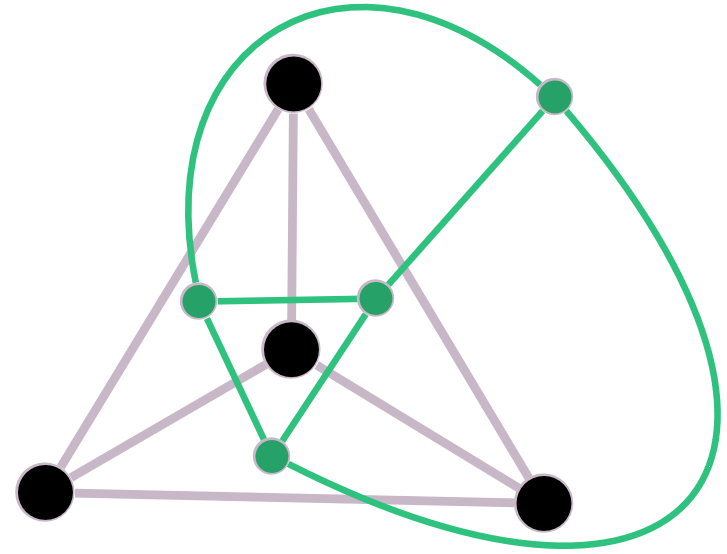
\includegraphics[width=4cm]{figures/duality/k4 with dual.png}
        \caption{A planar graph with its dual colored in green}
        \label{k4-with-dual}
    \end{subfigure}\hfill%
    \begin{subfigure}{.3\textwidth}
        \centering
        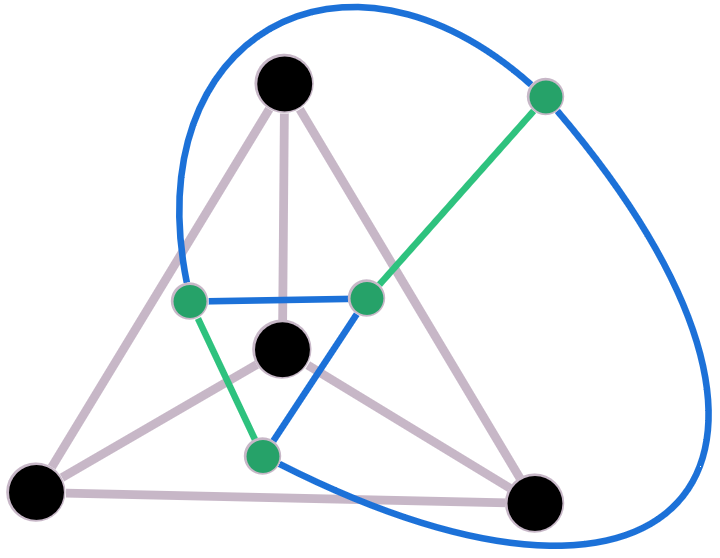
\includegraphics[width=4cm]{figures/duality/dual with cycle.png}
        \caption{A simple cycle in the dual, colored in blue}
        \label{dual-with-cycle}
    \end{subfigure}\hfill%
    \begin{subfigure}{.3\textwidth}
        \centering
        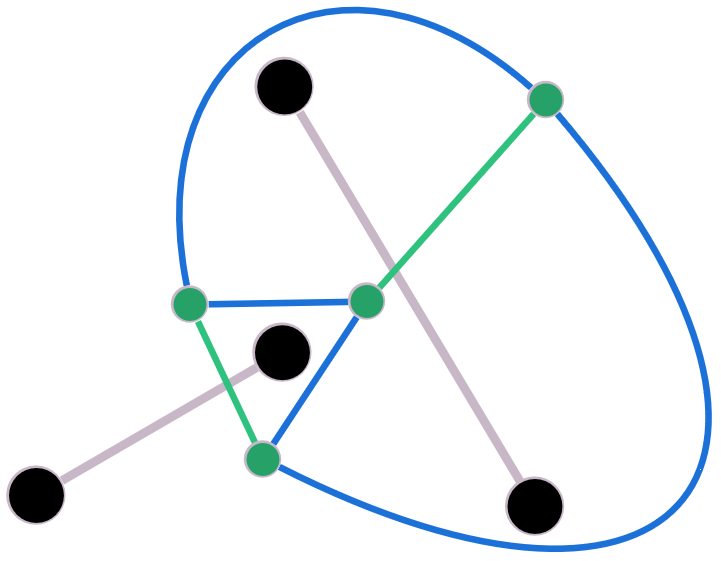
\includegraphics[width=4cm]{figures/duality/k4 cut in pieces.png}
        \caption{Deleting the edges that cross the dual's cycle cuts the graph in two}
        \label{k4-cut}
    \end{subfigure}
    \caption{A simple cycle in a dual graph always corresponds to a cut in the original graph.}
    \label{cycle-cut}
\end{figure}
